\documentclass[crop,tikz]{standalone}
\begin{document}
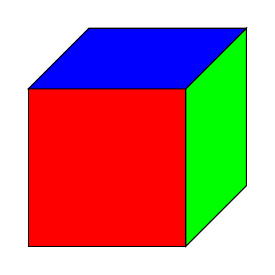
\begin{tikzpicture}
\pgfmathsetmacro{\cubex}{2}
\pgfmathsetmacro{\cubey}{2}
\pgfmathsetmacro{\cubez}{2}
\draw[black,fill=red] (0,0,0) -- ++(-\cubex,0,0) -- ++(0,-\cubey,0) -- ++(\cubex,0,0) -- cycle;
\draw[black,fill=green] (0,0,0) -- ++(0,0,-\cubez) -- ++(0,-\cubey,0) -- ++(0,0,\cubez) -- cycle;
\draw[black,fill=blue] (0,0,0) -- ++(-\cubex,0,0) -- ++(0,0,-\cubez) -- ++(\cubex,0,0) -- cycle;
\end{tikzpicture}
\end{document}
